\documentclass[11pt,a4paper]{article}

\usepackage[T1]{fontenc}
\usepackage[margin=1in]{geometry}
\usepackage{booktabs}
\usepackage{graphicx}
\usepackage{hyperref}
\usepackage{float}
\usepackage{array}

\newcolumntype{P}[1]{>{\raggedright\arraybackslash}p{#1}}
\graphicspath{{generated/figures/}{report/generated/figures/}}
\emergencystretch=2em

\newcommand{\inputgenerated}[1]{
    \IfFileExists{generated/#1}{
        \input{generated/#1}
    }{
        \input{report/generated/#1}
    }
}

\inputgenerated{summary_macros.tex}

\title{LLM-Based Code Smell Detection with Qwen2.5-Coder}
\author{
Nguyen Hoang Kien -- 20250735E\\
IT5433 -- Group 01\\
Topic: LLM-Based Code Smell Detection
}
\date{\today}

\begin{document}
\maketitle

\begin{abstract}
Code smells are recurring implementation or design patterns that may indicate maintainability problems. This report studies code smell detection as a multi-task binary classification problem over raw Java source code from the DeepLearningSmells dataset. Instead of reproducing the reference DeepSmells CNN-LSTM pipeline over tokenized inputs, the project fine-tunes Qwen2.5-Coder-3B-Instruct with QLoRA and compares it with a classical character TF-IDF LinearSVC baseline. The experiment uses four smell categories: Complex Method, Complex Conditional, Feature Envy, and Multifaceted Abstraction. Exact duplicate code fragments are removed before a fixed 70/15/15 train, validation, and test split. On the held-out test split, Qwen improves overall F1 from \baselinefione{} to \qwenfione{} and MCC from \baselinemcc{} to \qwenmcc{}. Prediction-level analysis shows that Qwen reduces total test errors from \baselineerrors{} to \qwenerrors{}, with the remaining errors concentrated in smells that require wider semantic or class-level context.
\end{abstract}

\section{Introduction}
Software systems become harder to maintain when implementation choices accumulate into overly complex methods, deeply nested conditions, misplaced responsibilities, or classes that mix unrelated concerns. These symptoms are commonly described as code smells \cite{fowler1999refactoring}. A smell is not necessarily a functional bug, but it can signal code that is difficult to understand, test, evolve, or refactor safely.

Automatic code smell detection is useful because manual inspection is expensive and inconsistent across large repositories. Traditional detectors usually rely on handcrafted metrics or static-analysis rules, while neural approaches attempt to learn smell-related patterns from code examples. The DeepLearningSmells repository and the DeepSmells reference work show that deep models can be trained for smell detection from processed code representations \cite{deeplearningsmells,deepsmells}. However, reproducing a reference pipeline alone would mainly test whether the original approach can be rerun.

This project instead asks whether a modern code-pretrained large language model can perform smell detection directly from raw source snippets. The report focuses on a Kaggle-feasible implementation: a character n-gram TF-IDF baseline and a QLoRA fine-tuned Qwen2.5-Coder-3B-Instruct model. The LLM is prompted with the programming language, target smell, short smell definition, and raw code, then trained to answer only \texttt{YES} or \texttt{NO}.

\inputgenerated{tables/research_questions.tex}

The main contributions are:
\begin{itemize}
    \item a raw-source-code LLM pipeline for Java code smell detection;
    \item a controlled comparison against a strong lexical TF-IDF baseline on the same test split;
    \item validation-based checkpoint selection without using the test set for model choice;
    \item prediction-level error analysis using confusion matrices, per-smell errors, and representative false positive and false negative patterns.
\end{itemize}

\section{Background and Related Work}
\subsection{Code Smells}
Code smells are maintainability indicators rather than formal correctness violations. A method may compile and pass tests while still being too long, too nested, or too dependent on foreign data. Fowler's refactoring catalog popularized the idea that recurring structural patterns can guide refactoring decisions \cite{fowler1999refactoring}. In this project, the target labels are binary: for a given source fragment and smell type, the model predicts whether the smell is present.

\inputgenerated{tables/smell_definitions.tex}

The four selected smells cover both local and broader design symptoms. Complex Method and Complex Conditional often have visible local signals such as long control flow, many statements, and nested branches. Feature Envy and Multifaceted Abstraction are harder because they may require understanding relationships between methods, fields, classes, and external objects.

\subsection{DeepLearningSmells and DeepSmells}
The dataset used in this work comes from DeepLearningSmells, which provides labeled examples and raw source archives for smell detection experiments \cite{deeplearningsmells}. The DeepSmells reference work uses a fusion of convolutional and recurrent neural networks over code representations \cite{deepsmells}. That line of work is important background because it shows that smell detection can be formulated as a supervised learning task.

This report does not attempt to reproduce the original DeepSmells architecture. Instead, the reference pipeline is used as background and the experiment changes the modeling assumption: the input is raw source code, and the main model is an instruction-tuned code LLM adapted with parameter-efficient fine-tuning.

\subsection{LLMs and Parameter-Efficient Fine-Tuning}
Qwen2.5-Coder is a code-specialized model family designed for code generation and code understanding tasks \cite{qwen25coder,qwen25coder3b}. A full fine-tuning run of a multi-billion-parameter model is expensive on Kaggle GPUs, so this project uses LoRA-style adapter training and 4-bit quantization. LoRA updates a small set of low-rank matrices instead of all base model weights \cite{hu2022lora}. QLoRA further reduces memory usage by loading the base model in 4-bit precision while training adapters \cite{dettmers2023qlora}. This makes the experiment feasible on Kaggle T4 hardware while still adapting the model to the target task.

\section{Dataset and Preprocessing}
The experiment uses the Java portion of the DeepLearningSmells raw source archives. The pre-tokenized \texttt{tokenizer\_*} data is intentionally not used for the LLM pipeline. Each final row contains the language, target smell, smell definition, raw source code, binary label, source path, split name, and code hash. A single multi-task dataset is built by combining all four smell-specific tasks.

Before splitting, exact duplicate code fragments are removed by hashing the code text. This is important because duplicate fragments appearing in both training and test sets would inflate performance. After duplicate removal, each smell task is balanced by sampling up to 1,500 positive and 1,500 negative examples. The split is then fixed once and reused for all models, with 70\% training, 15\% validation, and 15\% testing.

\inputgenerated{tables/dataset_split_summary.tex}

The final held-out test set contains 1,700 examples. Multifaceted Abstraction has fewer total examples than the other smells because fewer positive samples remain after filtering and balancing. This sampling strategy does not represent real deployment prevalence, where clean code may be much more common than smelly code. It is used here to create a fair supervised learning benchmark and to prevent accuracy from being dominated by the majority class.

\section{Methodology}
\subsection{Problem Formulation}
Each example is treated as a binary classification instance conditioned on a target smell. Given source code \(x\), smell type \(s\), and short smell definition \(d\), the model predicts \(y \in \{0,1\}\), where \(1\) means the smell is present. Conditioning on the smell name and definition allows one Qwen adapter to handle all four smell tasks instead of training a separate model for each smell.

\subsection{TF-IDF Baseline}
The baseline uses a character-level TF-IDF vectorizer with 3 to 5 character n-grams and a class-balanced LinearSVC classifier. Character n-grams are a strong baseline for source code because they capture local lexical patterns such as keywords, operators, indentation-like formatting, identifier fragments, and repeated API names. The baseline does not understand program semantics, but it is fast, deterministic, and competitive on many text classification tasks.

\subsection{Qwen Prompt and Answer-Token Training}
The LLM method converts each sample into an instruction prompt:
\begin{verbatim}
You are a code smell detection model.

Language: Java
Target smell: <smell>
Definition: <short smell definition>

Code:
<source code>

Answer only YES or NO.
\end{verbatim}

During supervised fine-tuning, the prompt tokens are masked and the loss is applied only to the answer tokens \texttt{YES} or \texttt{NO}. This keeps the task close to binary classification while using the instruction-following format expected by the model. At inference time, the model score is computed from the relative probability of \texttt{YES} and \texttt{NO}; the default threshold is fixed at 0.5 and is not tuned on the test set.

\subsection{Checkpoint Selection}
Trainer validation loss was disabled because it caused memory spikes on Kaggle T4 GPUs. Instead, the training process saves checkpoints periodically. After training, each candidate checkpoint is loaded and evaluated on the validation split using the same YES/NO inference procedure used for final testing. The checkpoint with the best validation MCC is selected, with validation F1 as the tie-breaker. The test split is evaluated exactly once using the selected checkpoint.

\section{Experimental Setup}
All experiments use the same fixed split and seed so that the baseline and Qwen results are directly comparable. The main model is Qwen2.5-Coder-3B-Instruct with QLoRA adapters. Training was run on Kaggle T4 GPUs under notebook time and memory constraints.

\inputgenerated{tables/hyperparameters.tex}

\inputgenerated{tables/experiment_metadata.tex}

Evaluation uses accuracy, precision, recall, F1, Matthews correlation coefficient (MCC), and ROC-AUC. Accuracy reports the fraction of correct predictions. Precision measures how many predicted smells are true smells, while recall measures how many true smells are found. F1 summarizes the precision-recall tradeoff. MCC is emphasized because it uses true positives, true negatives, false positives, and false negatives together, making it more robust than accuracy when class distributions differ. ROC-AUC measures ranking quality from model scores and is less dependent on the fixed YES/NO threshold.

\section{Implementation and Reproducibility}
The implementation is designed for Kaggle rather than a local workstation. The notebook is self-contained and does not require a separate Python module. This matters because Kaggle notebooks are easiest to share and rerun when the data, configuration, training logic, evaluation code, and report exports are kept in one executable artifact.

The raw DeepLearningSmells archives contain many files, so the notebook does not blindly extract the full archive contents. It first builds an index from the label metadata, samples the rows needed for the configured experiment, and extracts only the selected raw source files. This reduces storage pressure and avoids unnecessary I/O on Kaggle. The dataset split is written to disk so that all models use the same train, validation, and test assignments.

Long training jobs are separated from evaluation. During training, the notebook saves LoRA checkpoints and live training logs. For Kaggle reliability, checkpoints can also be backed up to a private Kaggle Dataset, which avoids losing all progress if an interactive session disconnects. After training, the evaluation-only mode restores the selected checkpoints, computes validation checkpoint metrics, chooses the best adapter, and then evaluates the test split exactly once.

The final artifacts include aggregate metrics, prediction-level outputs, checkpoint validation metrics, confusion matrices, LaTeX-ready tables, and the training loss curve. This makes the experiment auditable: the reported numbers are not copied manually from notebook cells, but exported from the same evaluation pipeline used to create the figures and tables in this report.

\section{Results}
\subsection{Overall Performance}
\inputgenerated{tables/overall_metrics.tex}

Qwen2.5-Coder-3B QLoRA substantially outperforms the TF-IDF baseline on the held-out test split. Overall F1 increases from \baselinefione{} to \qwenfione{}, and MCC increases from \baselinemcc{} to \qwenmcc{}. The improvement is visible not only in threshold-based metrics, but also in ROC-AUC, which indicates that Qwen produces better ranking scores across the test examples.

\inputgenerated{tables/confusion_summary.tex}

\begin{figure}[H]
    \centering
    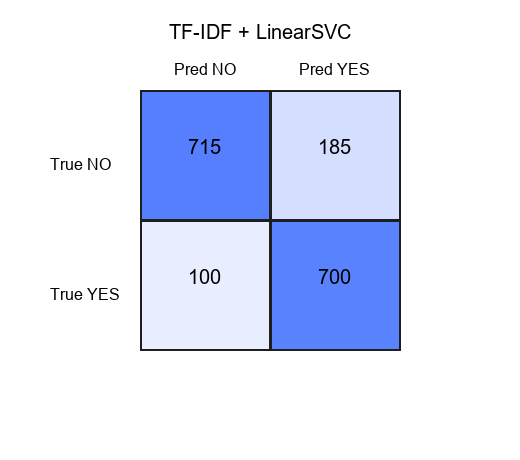
\includegraphics[width=0.44\textwidth]{confusion_matrix_baseline.png}
    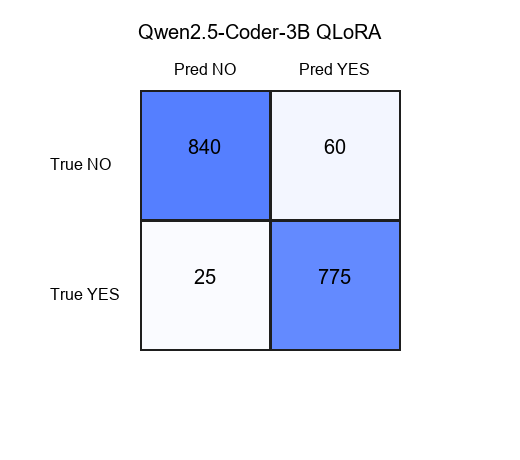
\includegraphics[width=0.44\textwidth]{confusion_matrix_qwen3b.png}
    \caption{Confusion matrices for the baseline and Qwen2.5-Coder-3B QLoRA.}
    \label{fig:confusion-matrices}
\end{figure}

The confusion matrices show that Qwen reduces both false positives and false negatives. The baseline makes \baselineerrors{} total errors, while Qwen makes \qwenerrors{}. This is important because a practical smell detector should avoid both missing problematic code and overwhelming developers with false alarms.

\subsection{Per-Smell Results}
\inputgenerated{tables/per_smell_metrics.tex}

The strongest Qwen results occur on Complex Conditional and Complex Method. These smells have local evidence that is often visible within a single code fragment, such as nested branches, long statement sequences, repeated condition checks, or broad method bodies. Qwen also improves Feature Envy and Multifaceted Abstraction, but those categories remain more difficult. They often depend on whether behavior belongs to another class or whether a class has mixed responsibilities, which can require context outside the provided snippet.

\begin{figure}[H]
    \centering
    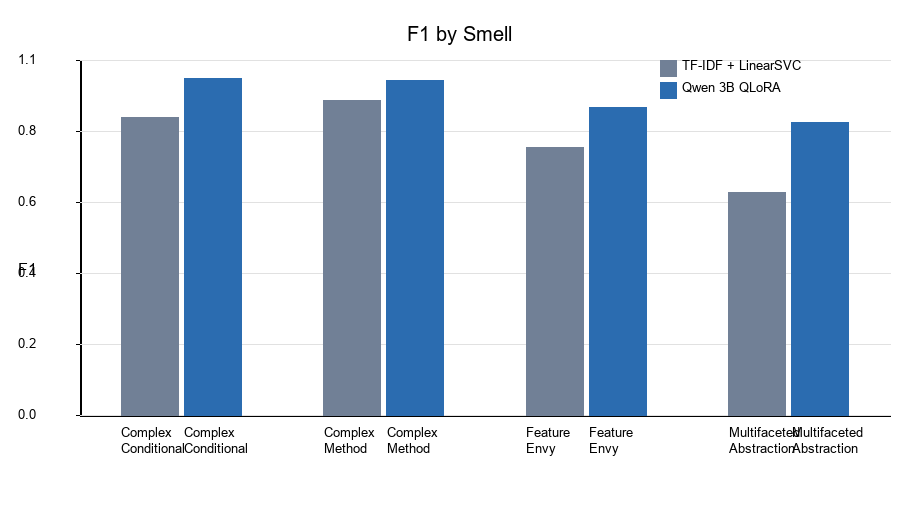
\includegraphics[width=0.48\textwidth]{f1_by_smell.png}
    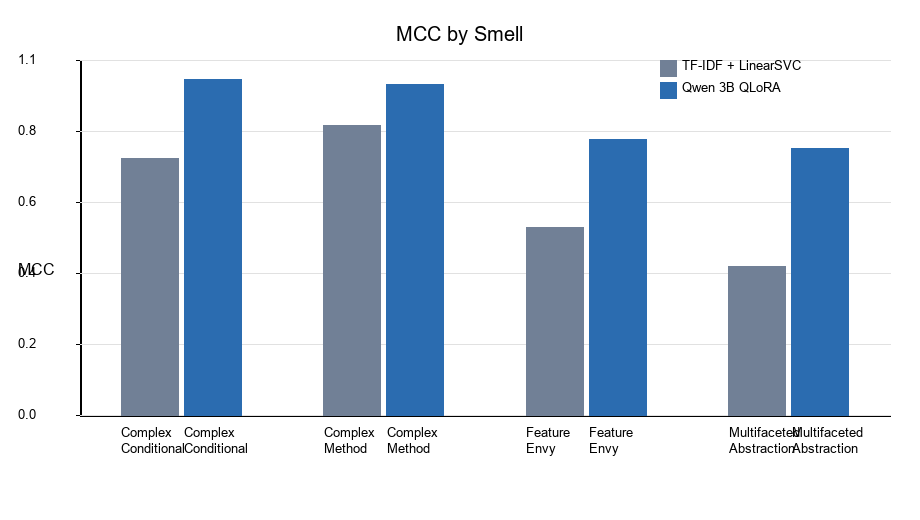
\includegraphics[width=0.48\textwidth]{mcc_by_smell.png}
    \caption{F1 and MCC by smell category.}
    \label{fig:smell-bars}
\end{figure}

\subsection{Checkpoint Selection and Training Behavior}
\inputgenerated{tables/checkpoint_selection.tex}

The final adapter at step \beststep{} is selected by validation MCC. The selection process avoids choosing a checkpoint based on test performance. Because the validation MCC and F1 of the final adapter are slightly higher than the saved intermediate checkpoints, the final adapter is used for the final test report.

\begin{figure}[H]
    \centering
    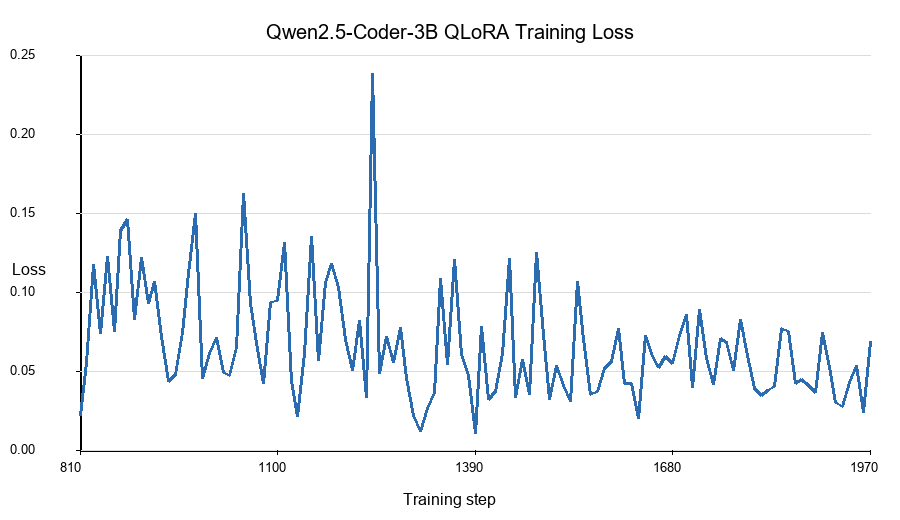
\includegraphics[width=0.75\textwidth]{training_loss_curve.png}
    \caption{Training loss during QLoRA fine-tuning.}
    \label{fig:training-loss}
\end{figure}

The training loss decreases strongly during fine-tuning, which indicates that the adapter learns the target answer format and dataset-specific decision boundary. This alone does not prove generalization, so the validation-checkpoint procedure and held-out test split are necessary. The high validation and test metrics suggest that the model does not merely memorize training labels, although near-duplicate code remains a possible threat.

\section{Error Analysis}
\inputgenerated{tables/error_count_by_smell.tex}

Prediction-level errors provide a more useful view than aggregate metrics alone. Qwen reduces errors for every smell category. Complex Conditional drops to only two errors and Complex Method to five errors. The largest remaining counts are Feature Envy and Multifaceted Abstraction, with 44 and 34 errors respectively.

False negatives occur when a smelly sample is predicted as clean. For Feature Envy, this can happen when the snippet contains external object interactions but does not clearly reveal whether the method depends more on foreign data than local state. For Multifaceted Abstraction, false negatives often occur when the local fragment looks like ordinary class infrastructure, while the responsibility mixing only becomes visible at class or project scope.

False positives occur when clean samples contain surface patterns that resemble smell indicators. A UI class with many configuration fields can look like a multifaceted abstraction. A method that calls model, view, or service objects can resemble Feature Envy even if those dependencies are normal for the class role. These errors show that Qwen uses richer code cues than the TF-IDF baseline, but it is still limited by the snippet-level input.

\inputgenerated{tables/sample_errors_qwen3b.tex}

\section{Discussion}
The main result is that Qwen2.5-Coder-3B QLoRA performs much better than a strong lexical baseline on this sampled Java benchmark. The gain is plausible because the LLM has been pretrained on code and can combine lexical, syntactic, and instruction-level signals. The smell definition in the prompt also gives the model task context at inference time, while the baseline only receives the raw text.

However, the result should be interpreted carefully. The experiment is a controlled held-out test over a balanced sample, not a production deployment study. Real repositories may have different smell prevalence, coding style, generated code, framework usage, and duplication patterns. A detector with high F1 on this benchmark may still need calibration and human review before being used in a development workflow.

The experiment also suggests that LLM-based smell detection is most suitable when the smell evidence is visible in the available context. Complex Method and Complex Conditional fit that condition well. Feature Envy and Multifaceted Abstraction would likely benefit from repository-level information, such as class fields, method call graphs, ownership of accessed data, and neighboring files.

\section{Threats to Validity}
The first threat is label quality. The dataset labels are generated from existing detection rules and may contain noise or tool-specific bias. A model can learn the rule patterns behind the labels without fully matching human maintainability judgments.

The second threat is sampling. Balanced sampling improves training stability and metric interpretability, but it changes the natural class distribution. Therefore, the reported accuracy, precision, and recall should not be read as real-world deployment rates.

The third threat is data leakage through near duplicates. Exact duplicate code fragments are removed before splitting, but near-duplicate code may remain across repositories or generated files. This can inflate generalization estimates if train and test examples are highly similar.

The fourth threat is context truncation. Long source files are truncated to fit the 2048-token LLM context window. Truncation can remove evidence needed for Feature Envy or Multifaceted Abstraction, especially when the decisive information appears outside the visible fragment.

The final threat is model and hardware specificity. The result is based on Qwen2.5-Coder-3B-Instruct with QLoRA under Kaggle constraints. Different code LLMs, thresholds, prompts, sequence lengths, or repository-level inputs may produce different results.

\section{Conclusion and Future Work}
This report presents an LLM-based code smell detection experiment over raw Java source code. Qwen2.5-Coder-3B with QLoRA achieves substantially stronger held-out test performance than TF-IDF + LinearSVC, improving overall F1 from \baselinefione{} to \qwenfione{} and reducing total test errors from \baselineerrors{} to \qwenerrors{}. The improvement is strongest for smells with local syntactic evidence and weaker for smells that require broader semantic context.

Future work should extend the input beyond single snippets by adding class-level context, repository metadata, and call or field access information. Another useful direction is threshold calibration on validation data, which may reduce false positives for developer-facing tools. Finally, the same framework can be extended to CSharp or other languages to test whether instruction-tuned code LLMs generalize across language ecosystems.

\bibliographystyle{plain}
\bibliography{references}

\end{document}
